\section{Datasety chodců} 
V~průběhu let bylo shromážděno nespočet trénovacích sad pro chodce, které jsou veřejně dostupné na internetu. Všechny mají rozdílné charakteristiky, slabé a~silné stránky. 

Sada INRIA \cite{inria} patří mezi nejstarší sady. Ačkoliv obsahuje poměrně málo vzorků, přináší díky tomu vysokou kvalitu anotací chodců v~různých prostředích, což je většinou hlavní důvod, proč je tato sada vybrána pro trénování. Na rozdíl sady ETH \cite{eth} a~TUD-Brussels \cite{tudbrussels} patří mezi středně velké video sady. Další známou trénovací sadou je Daimler--Mono \cite{daimler}, kterou nelze použít pro všechny metodiky, poněvadž poskytuje vzorky v~odstínech šedi. Sady ETH, KITTI \cite{kitti} a~Daimler-Stereo \cite{daimlerstereo} poskytují stereofonní informace. Na obrázku \ref{fig:daimler_stereo} je ukázka tréninkové a~testovací sady Daimler-Stereo. 

\begin{figure}[H]
\centering
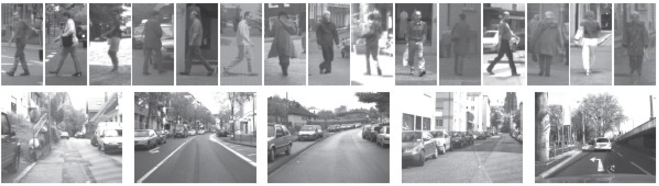
\includegraphics[width=16cm]{figures/daimler_stereo}
\caption{Ukázka trénovací a~testovací sady Daimler-Stereo \cite{daimlerstereo}}
\label{fig:daimler_stereo}
\end{figure}

V~dnešní době převládají Caltech-USA \cite{caltech} a~KITTI jako trénovací sady pro chodce. Obě poskytují poměrně velký počet vzorků. Caltech-USA vyniká počtem možných využití a~obsahuje více než 2300 jedinečných anotací chodců. KITTI zase předčí svou testovací sadou, která je více rozmanitější, ale na druhou stranu se tato sada nepoužívá tak často. V~roce 2014 vznikl projekt PETA (Pedestrian Attribute dataset)\cite{peta}. Tento projekt kombinuje mnoho trénovacích sad a~vytváří tak jednu velkou a~rozmanitou sadu, která usnadnuje učení robustních detektorů s~dobrým výkonem.

V~této práci používám převážně trénovací sadu CUHK01 \cite{cuhk}, sadu Das \cite{sudipdas} a~jako negativní sadu Daimler--Mono \cite{daimler}. Tato negativní sada se vyskytuje v~podobě fotografií zachycené kamerou při jezdě autem, bylo jí tedy nutné před použítím zpracovat. 

